% Created by tikzDevice version 0.12.6 on 2026-08-03 04:28:52
% !TEX encoding = UTF-8 Unicode
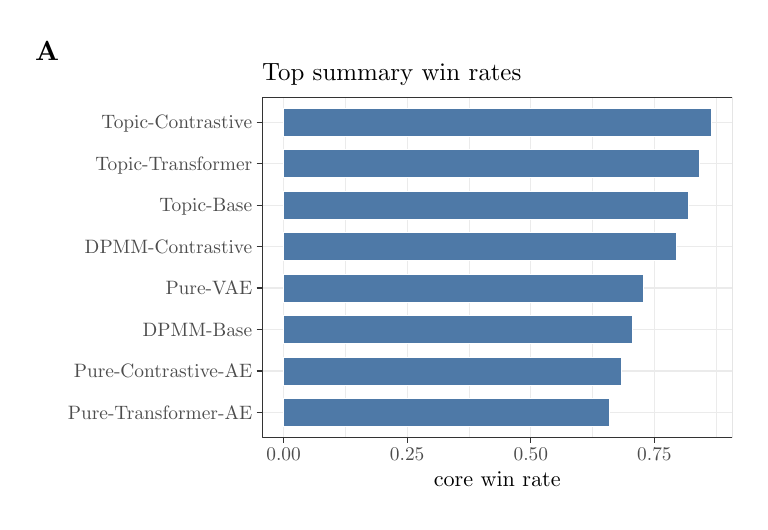
\begin{tikzpicture}[x=1pt,y=1pt]
\definecolor{fillColor}{RGB}{255,255,255}
\path[use as bounding box,fill=fillColor,fill opacity=0.00] (0,0) rectangle (257.30,171.36);
\begin{scope}
\path[clip] (  0.72,  1.87) rectangle (256.58,169.49);
\definecolor{drawColor}{RGB}{255,255,255}
\definecolor{fillColor}{RGB}{255,255,255}

\path[draw=drawColor,line width= 0.4pt,line join=round,line cap=round,fill=fillColor] (  0.72,  1.87) rectangle (256.58,169.49);
\end{scope}
\begin{scope}
\path[clip] ( 84.74, 23.34) rectangle (254.58,146.20);
\definecolor{fillColor}{RGB}{255,255,255}

\path[fill=fillColor] ( 84.74, 23.34) rectangle (254.58,146.20);
\definecolor{drawColor}{gray}{0.92}

\path[draw=drawColor,line width= 0.2pt,line join=round] (114.80, 23.34) --
	(114.80,146.20);

\path[draw=drawColor,line width= 0.2pt,line join=round] (159.48, 23.34) --
	(159.48,146.20);

\path[draw=drawColor,line width= 0.2pt,line join=round] (204.15, 23.34) --
	(204.15,146.20);

\path[draw=drawColor,line width= 0.2pt,line join=round] (248.82, 23.34) --
	(248.82,146.20);

\path[draw=drawColor,line width= 0.4pt,line join=round] ( 84.74, 32.33) --
	(254.58, 32.33);

\path[draw=drawColor,line width= 0.4pt,line join=round] ( 84.74, 47.31) --
	(254.58, 47.31);

\path[draw=drawColor,line width= 0.4pt,line join=round] ( 84.74, 62.29) --
	(254.58, 62.29);

\path[draw=drawColor,line width= 0.4pt,line join=round] ( 84.74, 77.28) --
	(254.58, 77.28);

\path[draw=drawColor,line width= 0.4pt,line join=round] ( 84.74, 92.26) --
	(254.58, 92.26);

\path[draw=drawColor,line width= 0.4pt,line join=round] ( 84.74,107.24) --
	(254.58,107.24);

\path[draw=drawColor,line width= 0.4pt,line join=round] ( 84.74,122.22) --
	(254.58,122.22);

\path[draw=drawColor,line width= 0.4pt,line join=round] ( 84.74,137.21) --
	(254.58,137.21);

\path[draw=drawColor,line width= 0.4pt,line join=round] ( 92.46, 23.34) --
	( 92.46,146.20);

\path[draw=drawColor,line width= 0.4pt,line join=round] (137.14, 23.34) --
	(137.14,146.20);

\path[draw=drawColor,line width= 0.4pt,line join=round] (181.81, 23.34) --
	(181.81,146.20);

\path[draw=drawColor,line width= 0.4pt,line join=round] (226.49, 23.34) --
	(226.49,146.20);
\definecolor{drawColor}{RGB}{255,255,255}
\definecolor{fillColor}{RGB}{78,121,167}

\path[draw=drawColor,line width= 0.2pt,fill=fillColor] ( 92.46,132.11) rectangle (246.86,142.30);

\path[draw=drawColor,line width= 0.2pt,fill=fillColor] ( 92.46,117.13) rectangle (242.75,127.32);

\path[draw=drawColor,line width= 0.2pt,fill=fillColor] ( 92.46,102.15) rectangle (238.64,112.33);

\path[draw=drawColor,line width= 0.2pt,fill=fillColor] ( 92.46, 87.16) rectangle (234.53, 97.35);

\path[draw=drawColor,line width= 0.2pt,fill=fillColor] ( 92.46, 72.18) rectangle (222.38, 82.37);

\path[draw=drawColor,line width= 0.2pt,fill=fillColor] ( 92.46, 57.20) rectangle (218.45, 67.39);

\path[draw=drawColor,line width= 0.2pt,fill=fillColor] ( 92.46, 42.22) rectangle (214.34, 52.40);

\path[draw=drawColor,line width= 0.2pt,fill=fillColor] ( 92.46, 27.23) rectangle (210.23, 37.42);
\definecolor{drawColor}{gray}{0.20}

\path[draw=drawColor,line width= 0.4pt,line join=round,line cap=round] ( 84.74, 23.34) rectangle (254.58,146.20);
\end{scope}
\begin{scope}
\path[clip] (  0.00,  0.00) rectangle (257.30,171.36);
\definecolor{drawColor}{gray}{0.30}

\node[text=drawColor,anchor=base east,inner sep=0pt, outer sep=0pt, scale=  0.70] at ( 81.14, 29.92) {Pure-Transformer-AE};

\node[text=drawColor,anchor=base east,inner sep=0pt, outer sep=0pt, scale=  0.70] at ( 81.14, 44.90) {Pure-Contrastive-AE};

\node[text=drawColor,anchor=base east,inner sep=0pt, outer sep=0pt, scale=  0.70] at ( 81.14, 59.88) {DPMM-Base};

\node[text=drawColor,anchor=base east,inner sep=0pt, outer sep=0pt, scale=  0.70] at ( 81.14, 74.86) {Pure-VAE};

\node[text=drawColor,anchor=base east,inner sep=0pt, outer sep=0pt, scale=  0.70] at ( 81.14, 89.85) {DPMM-Contrastive};

\node[text=drawColor,anchor=base east,inner sep=0pt, outer sep=0pt, scale=  0.70] at ( 81.14,104.83) {Topic-Base};

\node[text=drawColor,anchor=base east,inner sep=0pt, outer sep=0pt, scale=  0.70] at ( 81.14,119.81) {Topic-Transformer};

\node[text=drawColor,anchor=base east,inner sep=0pt, outer sep=0pt, scale=  0.70] at ( 81.14,134.80) {Topic-Contrastive};
\end{scope}
\begin{scope}
\path[clip] (  0.00,  0.00) rectangle (257.30,171.36);
\definecolor{drawColor}{gray}{0.20}

\path[draw=drawColor,line width= 0.4pt,line join=round] ( 82.74, 32.33) --
	( 84.74, 32.33);

\path[draw=drawColor,line width= 0.4pt,line join=round] ( 82.74, 47.31) --
	( 84.74, 47.31);

\path[draw=drawColor,line width= 0.4pt,line join=round] ( 82.74, 62.29) --
	( 84.74, 62.29);

\path[draw=drawColor,line width= 0.4pt,line join=round] ( 82.74, 77.28) --
	( 84.74, 77.28);

\path[draw=drawColor,line width= 0.4pt,line join=round] ( 82.74, 92.26) --
	( 84.74, 92.26);

\path[draw=drawColor,line width= 0.4pt,line join=round] ( 82.74,107.24) --
	( 84.74,107.24);

\path[draw=drawColor,line width= 0.4pt,line join=round] ( 82.74,122.22) --
	( 84.74,122.22);

\path[draw=drawColor,line width= 0.4pt,line join=round] ( 82.74,137.21) --
	( 84.74,137.21);
\end{scope}
\begin{scope}
\path[clip] (  0.00,  0.00) rectangle (257.30,171.36);
\definecolor{drawColor}{gray}{0.20}

\path[draw=drawColor,line width= 0.4pt,line join=round] ( 92.46, 21.34) --
	( 92.46, 23.34);

\path[draw=drawColor,line width= 0.4pt,line join=round] (137.14, 21.34) --
	(137.14, 23.34);

\path[draw=drawColor,line width= 0.4pt,line join=round] (181.81, 21.34) --
	(181.81, 23.34);

\path[draw=drawColor,line width= 0.4pt,line join=round] (226.49, 21.34) --
	(226.49, 23.34);
\end{scope}
\begin{scope}
\path[clip] (  0.00,  0.00) rectangle (257.30,171.36);
\definecolor{drawColor}{gray}{0.30}

\node[text=drawColor,anchor=base,inner sep=0pt, outer sep=0pt, scale=  0.70] at ( 92.46, 14.92) {0.00};

\node[text=drawColor,anchor=base,inner sep=0pt, outer sep=0pt, scale=  0.70] at (137.14, 14.92) {0.25};

\node[text=drawColor,anchor=base,inner sep=0pt, outer sep=0pt, scale=  0.70] at (181.81, 14.92) {0.50};

\node[text=drawColor,anchor=base,inner sep=0pt, outer sep=0pt, scale=  0.70] at (226.49, 14.92) {0.75};
\end{scope}
\begin{scope}
\path[clip] (  0.00,  0.00) rectangle (257.30,171.36);
\definecolor{drawColor}{RGB}{0,0,0}

\node[text=drawColor,anchor=base,inner sep=0pt, outer sep=0pt, scale=  0.80] at (169.66,  5.64) {core win rate};
\end{scope}
\begin{scope}
\path[clip] (  0.00,  0.00) rectangle (257.30,171.36);
\definecolor{drawColor}{RGB}{0,0,0}

\node[text=drawColor,anchor=base west,inner sep=0pt, outer sep=0pt, scale=  0.90] at ( 84.74,152.18) {Top summary win rates};
\end{scope}
\begin{scope}
\path[clip] (  0.00,  0.00) rectangle (257.30,171.36);
\definecolor{drawColor}{RGB}{0,0,0}

\node[text=drawColor,anchor=base,inner sep=0pt, outer sep=0pt, scale=  1.00] at (  7.07,159.49) {\bfseries A};
\end{scope}
\end{tikzpicture}
